\documentclass[10pt]{article}
\usepackage[polish]{babel}
\usepackage[utf8]{inputenc}
\usepackage[T1]{fontenc}
\usepackage{amsmath}
\usepackage{amsfonts}
\usepackage{amssymb}
\usepackage[version=4]{mhchem}
\usepackage{stmaryrd}
\usepackage{graphicx}
\usepackage[export]{adjustbox}
\graphicspath{ {./images/} }

\title{MATEMATYKA-klasa 2-(pp) }

\author{}
\date{}


\begin{document}
\maketitle
\(\qquad\)

MAJ 2017

\section*{LSCDN}
\section*{Instrukcja dla zdającego}
MATEMATYKA- klasa 2-(pp)

Czas pracy:\\
170 minut

\begin{enumerate}
  \item Sprawdź, czy arkusz zawiera 14 stron (zadania 1-34). Ewentualny brak zgłoś przewodniczącemu zespołu nadzorującego egzamin.
  \item Rozwiązania zadań i odpowiedzi zamieść w miejscu na to przeznaczonym.
  \item Odpowiedzi do zadań zamkniętych (1-25) przenieś na kartę odpowiedzi, zaznaczając je w części karty przeznaczonej dla zdającego. Zamaluj pola do tego przeznaczone. Błędne zaznaczenie otocz kółkiem izaznacz właściwe.
  \item Pamiętaj, że pominięcie argumentacji lub istotnych obliczeń w rozwiązaniu zadania otwartego (26-34) może spowodować, że za to rozwiązanie nie otrzymasz pełnej liczby punktów.
  \item Pisz czytelnie i używaj tylko długopisu lub pióra z czarnym tuszem lub atramentem.
  \item Nie używaj korektora, a błędne zapisy wyraźnie przekreśl.
  \item Pamiętaj, że zapisy w brudnopisie nie będą oceniane.
  \item Możesz korzystać z zestawu wzorów matematycznych, cyrkla i linijki oraz kalkulatora prostego.
  \item Nie wpisuj żadnych znaków w części przeznaczonej dla egzaminatora.
\end{enumerate}

\section*{Zadanie 1. (1p)}
Jeżeli \(a=\sqrt[3]{8} \cdot 2^{\frac{1}{2}} i \quad b=\left(\frac{1}{8}\right)^{-\frac{1}{3}}\), to wartość wyrażenia \(\left(\frac{a}{b}\right)^{-1}\) jest równa\\
A. \(2^{-\frac{1}{2}}\)\\
B. \(2^{\frac{1}{2}}\)\\
C. \(-2^{\frac{1}{2}}\)\\
D. \(-2^{-\frac{1}{2}}\)

Zadanie 2. (1p)\\
Jeżeli liczba 91 jest o 40\% większa od liczby x, to liczba x jest równa\\
A. 72\\
B. 70\\
C. 68\\
D. 65

\section*{Zadanie 3. (1p)}
Wartość wyrażenia \(\left|\frac{2-2 \sqrt{2}}{2-\sqrt{2}}\right|\) jest równa\\
A. \(2 \sqrt{2}\)\\
B. \(\sqrt{2}\)\\
C. \(2-\sqrt{2}\)\\
D. 2

\section*{Zadanie 4. (1p)}
Jeżeli \(\frac{a}{b}=3\), to wartość wyrażenia \(\frac{3(a-b)}{a}\) jest równa\\
A. \(\frac{1}{2}\)\\
B. \(\frac{3}{2}\)\\
C. 2\\
D. 3

Zadanie 5. (1p)\\
Wartość wyrażenia \(2 \log _{3} 2-2 \log _{3} \frac{2}{3}\) jest równa\\
A. 4\\
B. 2\\
C. 3\\
D. 1

\section*{Zadanie 6. (1p)}
Funkcja kwadratowa \(f(x)=-3(x-6)(4-x)\) jest malejąca w przedziale\\
A. \(x \in(-\infty, 6)\)\\
B. \(x \in\langle 4,+\infty)\)\\
C. \(x \in(-\infty, 5\rangle\)\\
D. \(x \in(5,+\infty)\)

\section*{Zadanie 7. (1p)}
Wartość wyrażenia \(\left(\frac{\cos 150^{\circ}}{\sin 60^{\circ}}-\sin 90^{\circ}\right)^{-2}\) jest równa\\
A. \(-\frac{1}{4}\)\\
B. -1\\
C. 1\\
D. \(\frac{1}{4}\)

\section*{Zadanie 8. (1p)}
Punkt S jest środkiem okręgu, na którym leżą punkty A, B i C (patrz rysunek). Jeśli \(|A C|=|B C|\) i miara kąta wypukłego \(A S B=124^{\circ}\), to kąt wypukły \(S A C\) jest równy\\
A. \(32^{\circ}\)\\
B. \(31^{\circ}\)\\
C. \(30^{\circ}\)\\
D. \(29^{\circ}\)\\
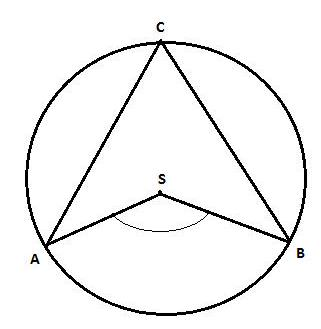
\includegraphics[max width=\textwidth, center]{2024_11_21_3747d4b97b2de24458ddg-02}

\section*{BRUDNOPIS}
Zadanie 9. (1p)\\
Kąty trójkąta tworzą ciąg geometryczny o ilorazie 4. Miara największego z nich jest równa\\
A. \(\frac{1}{7} \cdot 360^{\circ}\)\\
B. \(\frac{1}{7} \cdot 540^{\circ}\)\\
C. \(\frac{1}{7} \cdot 630^{\circ}\)\\
D. \(\frac{1}{7} \cdot 960^{\circ}\)

Zadanie 10. (1p)\\
Dziedziną funkcji \(f(x)=\frac{\sqrt{x-2}}{\sqrt{x-1}}\) jest przedział\\
A. \(x \in(-\infty, 1)\)\\
B. \(x \in\langle 2,+\infty)\)\\
C. \(x \in(-\infty, 2\rangle\)\\
D. \(x \in(1,+\infty)\)

\section*{Zadanie 11. (1p)}
Pole powierzchni trójkąta równoramiennego o ramionach długości 6 cm i kącie między nimi \(120^{\circ}\) jest równe\\
A. \(36 \mathrm{~cm}^{2}\)\\
B. \(18 \mathrm{~cm}^{2}\)\\
C. \(9 \sqrt{3} \mathrm{~cm}^{2}\)\\
D. \(9 \mathrm{~cm}^{2}\)

Zadanie 12. (1p)\\
Jeżeli \(f(x)=x+2\) i \(g(x)=f(x+3)-2\), to funkcja \(g(x)\) jest równa\\
A. \(-x+3\)\\
B. \(x-3\)\\
C. \(-x-3\)\\
D. \(x+3\)

Zadanie 13. (1p)\\
Dziedziną funkcji f jest przedział \((-5,8)\). Zatem dziedziną funkcji \(f(x-5)+1\) jest przedział:\\
A. \((0,13)\).\\
B. \((-10,3)\)\\
C. \((-4,9)\)\\
D. \((-6,7)\)

Zadanie 14. (1p)\\
Punkt \(A=(1,1)\) jest jednym z wierzchołków kwadratu \(A B C D\), a punkt \(S=(4,4)\) jest środkiem okręgu wpisanego w ten kwadrat. Przekątna tego kwadratu jest równa\\
A. \(8 \sqrt{2}\)\\
B. \(2 \sqrt{6}\)\\
C. \(6 \sqrt{2}\)\\
D. \(2 \sqrt{8}\)

\section*{Zadanie 15. (1p)}
O funkcji liniowej f wiadomo, że \(f(2)=3\) oraz punkt \(P=(4,2)\) należy do jej wykresu. Wzór funkcji f to\\
A. \(f(x)=\frac{1}{2} x+4\)\\
B. \(f(x)=-\frac{1}{2} x+4\)\\
C. \(f(x)=-\frac{1}{2} x-4\)\\
D. \(f(x)=\frac{1}{2} x-4\)

\section*{Zadanie 16. (1p)}
Długość odcinka zaznaczonego na rysunku literką x jest równa\\
A. \(2,4 \mathrm{~cm}\)\\
B. 3 cm\\
C. \(\frac{3}{4} \mathrm{~cm}\)\\
D. 2 cm\\
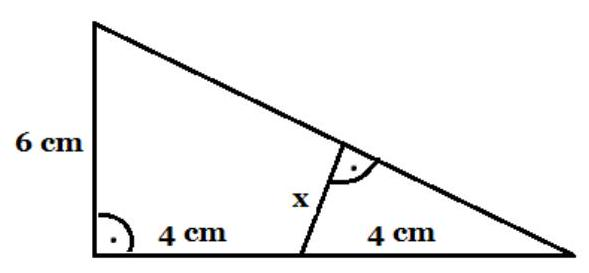
\includegraphics[max width=\textwidth, center]{2024_11_21_3747d4b97b2de24458ddg-04}

\section*{BRUDNOPIS}
\section*{Zadanie 17. (1p)}
Zbiorem wartości funkcji \(y=(x-2)(x+4)\) jest przedział\\
A. \(\langle-2,+\infty)\)\\
B. \(\langle 4,+\infty)\)\\
C. \(\langle-4,2\rangle\)\\
D. \(\langle-9,+\infty)\)

Zadanie 18. (1p)\\
Dany jest trzywyrazowy ciąg arytmetyczny \((x, 2 x-3,4 x-4)\). Stąd wynika, że \(x\) jest równy\\
A. -4\\
B. -3\\
C. -2\\
D. -1

Zadanie 19. (1p)\\
Wyrażenie \(\frac{1-\operatorname{tg}^{2} \alpha}{1+\operatorname{tg}^{2} \alpha}\) jest równe\\
A. 1\\
B. \(1-2 \sin ^{2} \alpha\)\\
C. 0\\
D. \(\cos ^{2} \alpha\)

\section*{Zadanie 20. (1p)}
Dla każdej liczby całkowitej dodatniej n , suma n początkowych wyrazów ciągu arytmetycznego \(\left(a_{n}\right)\) jest określona wzorem \(S_{n}=2 n^{2}+2 n\). Wtedy wyraz \(a_{2}\) jest równy\\
A. 5\\
B. 6\\
C. 7\\
D. 8

\section*{Zadanie 21. (1p)}
Najmniejszą liczbą całkowitą spełniającą nierówność \(\frac{x}{7}+\sqrt{2}>0\) jest\\
A. -11\\
B. -9\\
C. -7\\
D. 9

\section*{Zadanie 22. (1p)}
Liczby \(\{11,1,-9\}\) są trzema początkowymi wyrazami ciągu arytmetycznego \(\left(a_{n}\right)\), określonego dla liczb naturalnych \(n \geq 1\). Wzór ogólny tego ciągu ma postać\\
A. \(a_{n}=-10 n-21\)\\
B. \(a_{n}=-10 n-21\)\\
C. \(a_{n}=10 n+21\)\\
D. \(a_{n}=-10 n+21\)

\section*{Zadanie 23. (1p)}
Trzeci wyraz malejącego ciągu geometrycznego jest równy \(\frac{1}{4}\), a piąty \(\frac{1}{16}\). Iloraz tego ciągu jest równy\\
A. -2\\
B. \(-\frac{1}{2}\)\\
C. \(\frac{1}{2}\)\\
D. 2

Zadanie 24. (1p)\\
Punkt \(S=(2,7)\) jest środkiem odcinka AB, w którym \(B=(-1,3)\). Współrzędne punktu A są równe\\
A. \(A=(5,11)\)\\
B. \(A=\left(\frac{1}{2}, 5\right)\)\\
C. \(A=(1,10)\)\\
D. \(A=(-5,11)\)

Zadanie 25. (1p)\\
Do wykresu funkcji określonej wzorem \(f(x)=2^{x-1}+1\), należy punkt o współrzędnych\\
A. \(\left(0, \frac{1}{2}\right)\)\\
B. \((1,2)\)\\
C. \((2,4)\)\\
D. \((4,4)\)

\section*{BRUDNOPIS}
\section*{LUBELSKA PRÓBA PRZED MATURĄ 2017 - klasa 2 (pp)}
\section*{ZADANIA OTWARTE}
Rozwiqzania zadań o numerach od 26 do 34 należy zapisać w wyznaczonych miejscach pod treściq zadania (pamiętaj o udzieleniu odpowiedzi)

\section*{Zadanie 26. (2p)}
Wyznacz zbiór całkowitych rozwiązań nierówności \(\frac{x^{2}+9}{3}<3 x-3\).

Odpowiedź:\\
Zadanie 27. (2p)\\
Wykaż, ze dla dowolnych liczb rzeczywistych a, b prawdziwa jest nierówność \(a^{2}+b^{2} \geq 2(a+b-1)\).\\

\includegraphics[max width=\textwidth, center]{2024_11_21_3747d4b97b2de24458ddg-08}

Odpowiedź:

Zadanie 28. (2p)\\
Ile wyrazów ujemnych ma ciąg liczbowy określony wzorem \(a_{n}=n^{2}-2 n-24\) dla \(n \geq 1\) ?

Odpowiedź:

\section*{Zadanie 29. (2p)}
Rozwiąż równanie \(\frac{2-3 x}{1-2 x}=-\frac{1}{2}\).

\section*{Zadanie 30. (2p)}
Kąt \(\alpha\) jest ostry i \(\operatorname{tg} \alpha=\frac{4}{3}\). Oblicz \(\sin \alpha+\cos \alpha\).

\section*{Zadanie 31. (3p)}
Oblicz długości boków trójkąta prostokątnego o polu powierzchni równym 20, wiedząc, że długości jego przyprostokątnych różnią się o 6 .

\section*{Zadanie 32. (4p)}
W trójkącie prostokątnym ABC z wierzchołka kąta prostego poprowadzono odcinek CD taki, że \(D \in A B\). Trójkąt ADC jest równoboczny. Oblicz pole trójkąta \(A B C\), wiedząc, że jego obwód jest równy 6.\\
\(\qquad\)\\
Odpowiedź:\\
Zadanie 33. (4p)\\
Szósty wyraz ciągu arytmetycznego \(\left(a_{n}\right)\) jest o 6 mniejszy od czwartego wyrazu. Wyznacz wzór ogólny na n-ty wyraz ciągu \(\left(a_{n}\right)\), wiedząc, że ciąg \(\left(a_{1}, a_{3},-\frac{1}{2} a_{7}\right)\) jest geometryczny

Odpowiedź:

\section*{LUBELSKA PRÓBA PRZED MATURĄ 2017 - klasa 2 (pp)}
\section*{Zadanie 34. (4p)}
Dany jest trójkąt ABC, gdzie \(A=(-5,-2), B=(3,-1), C=(-1,6)\).\\
a) wyznacz równanie prostej zawierającej bok AC,\\
b) oblicz długość środkowej AD,\\
c) wyznacz równanie prostej zawierającej wysokość poprowadzoną z wierzchołka C ,\\
d) oblicz pole tego trójkąta.

Odpowiedź:

BRUDNOPIS

\section*{BRUDNOPIS}
KARTA ODPOWIEDZI\\
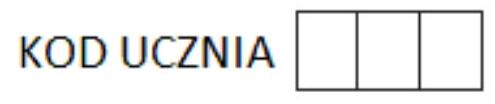
\includegraphics[max width=\textwidth, center]{2024_11_21_3747d4b97b2de24458ddg-14(1)}

Nazwisko i imię

Wypelnia piszący

\begin{center}
\begin{tabular}{|c|c|c|c|c|}
\hline
\begin{tabular}{c}
Nr \\
zaduia \\
\end{tabular} & A & B & C & D \\
\hline
1. & \(\square\) & \(\square\) & \(\square\) & \(\square\) \\
\hline
2. & \(\square\) & \(\square\) & \(\square\) & \(\square\) \\
\hline
3. & \(\square\) & \(\square\) & \(\square\) & \(\square\) \\
\hline
4. & \(\square\) & \(\square\) & \(\square\) & \(\square\) \\
\hline
5. & \(\square\) & \(\square\) & \(\square\) & \(\square\) \\
\hline
6. & \(\square\) & \(\square\) & \(\square\) & \(\square\) \\
\hline
7. & \(\square\) & \(\square\) & \(\square\) & \(\square\) \\
\hline
8. & \(\square\) & \(\square\) & \(\square\) & \(\square\) \\
\hline
9. & \(\square\) & \(\square\) & \(\square\) & \(\square\) \\
\hline
10. & \(\square\) & \(\square\) & \(\square\) & \(\square\) \\
\hline
11. & \(\square\) & \(\square\) & \(\square\) & \(\square\) \\
\hline
12. & \(\square\) & \(\square\) & \(\square\) & \(\square\) \\
\hline
13. & \(\square\) & \(\square\) & \(\square\) & \(\square\) \\
\hline
14. & \(\square\) & \(\square\) & \(\square\) & \(\square\) \\
\hline
15. & \(\square\) & \(\square\) & \(\square\) & \(\square\) \\
\hline
16. & \(\square\) & \(\square\) & \(\square\) & \(\square\) \\
\hline
17. & \(\square\) & \(\square\) & \(\square\) & \(\square\) \\
\hline
18. & \(\square\) & \(\square\) & \(\square\) & \(\square\) \\
\hline
19. & \(\square\) & \(\square\) & \(\square\) & \(\square\) \\
\hline
20. & \(\square\) & \(\square\) & \(\square\) & \(\square\) \\
\hline
21. & \(\square\) & \(\square\) & \(\square\) & \(\square\) \\
\hline
22. & \(\square\) & \(\square\) & \(\square\) & \(\square\) \\
\hline
23. & \(\square\) & \(\square\) & \(\square\) & \(\square\) \\
\hline
24. & \(\square\) & \(\square\) & \(\square\) & \(\square\) \\
\hline
25. & \(\square\) & \(\square\) & \(\square\) & \(\square\) \\
\hline
\end{tabular}
\end{center}

Razem \(\square\)

Wypelnia sprawdzający

\begin{center}
\begin{tabular}{|c|c|c|c|c|}
\hline
\begin{tabular}{c}
Nr \\
zadsuia \\
\end{tabular} & X & 0 & 1 & 2 \\
\hline
26. & \(\square\) & \(\square\) & \(\square\) & \(\square\) \\
\hline
27. & \(\square\) & \(\square\) & \(\square\) & \(\square\) \\
\hline
28. & \(\square\) & \(\square\) & \(\square\) & \(\square\) \\
\hline
29. & \(\square\) & \(\square\) & \(\square\) & \(\square\) \\
\hline
30. & \(\square\) & \(\square\) & \(\square\) & \(\square\) \\
\hline
\end{tabular}
\end{center}

Razem\\
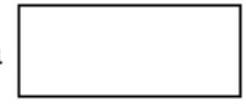
\includegraphics[max width=\textwidth, center]{2024_11_21_3747d4b97b2de24458ddg-14}

\begin{center}
\begin{tabular}{|c|c|c|c|c|c|c|c|}
\hline
\begin{tabular}{c}
Nr \\
zadaia \\
\end{tabular} & X & 0 & 1 & 2 & 3 & 4 & 5 \\
\hline\hline
31. & \(\square\) & \(\square\) & \(\square\) & \(\square\) & \(\square\) &  &  \\
\hline
32. & \(\square\) & \(\square\) & \(\square\) & \(\square\) & \(\square\) & \(\square\) &  \\
\hline
33. & \(\square\) & \(\square\) & \(\square\) & \(\square\) & \(\square\) & \(\square\) &  \\
\hline
34. & \(\square\) & \(\square\) & \(\square\) & \(\square\) & \(\square\) & \(\square\) &  \\
\hline
\end{tabular}
\end{center}

Razem\\
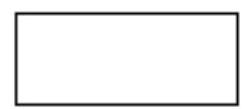
\includegraphics[max width=\textwidth, center]{2024_11_21_3747d4b97b2de24458ddg-14(2)}

\begin{center}
\begin{tabular}{|l|l|}
\hline
Suma punktów & Wynik w\% \\
\hline
 &  \\
 &  \\
\hline
\end{tabular}
\end{center}


\end{document}